% !TeX root = RJwrapper.tex
\title{A clustering algorithm to organize satellite hotspots data for the
purpose of tracking bushfires remotely}
\author{by Weihao Li, Emily Dodwell, and Dianne Cook}

\maketitle

\abstract{%
An abstract of less than 150 words.
}

\hypertarget{introduction}{%
\subsection{Introduction}\label{introduction}}

Bushfires are a major problem for Australia, and many other parts of the
globe. There is concern that as the climate becomes hotter, and drier,
that the impact of fires becomes much more severe and extensive. In
Australia, the 2019-2020 fires were the worst on record causing
extensive ecological damage, as well as damage to agricultural
resources, properties and infrastructure. The Wollemi pine, rare
prehistoric trees, required special forces intervention to prevent the
last stands in the world, in remote wilderness areas, from being turned
into ash.

Contributing to the problem is that many fires started in very remote
areas, locations deep into the temperate forests ignited by lightning,
that are virtually impossible to access or to monitor. Satellite data
provides a possible solution to this, particularly remotely sensed hot
spot data, which may be useful in detecting new ignitions and movements
of fires. Understanding fires in remote areas using satellite data may
provide some help in developing effective strategies for mitigating
bushfire impact.

This work addresses this topic. Using hot spot data, can we cluster in
space and time, in order to determine (1) points of ignition and (2)
track the movement of bush fires.

This paper is organised as follows. The next section provides an
introduction to the literature on spatiotemporal clustering and bush
fire modeling and dynamics. Section
\protect\hyperlink{algorithm}{Algorithm} describes the clustering
algorithm, and section \protect\hyperlink{application}{Application}
illustrates how the resulting data can be used to study bush fire
ignition.

\hypertarget{background}{%
\subsection{Background}\label{background}}

\hypertarget{spatiotemporal-clustering}{%
\subsubsection{Spatiotemporal
clustering}\label{spatiotemporal-clustering}}

\hypertarget{bushfire-modeling}{%
\subsubsection{Bushfire modeling}\label{bushfire-modeling}}

\hypertarget{algorithm}{%
\subsection{Algorithm}\label{algorithm}}

\hypertarget{data-pre-processing}{%
\subsubsection{Data pre-processing}\label{data-pre-processing}}

\begin{Schunk}
\begin{figure}
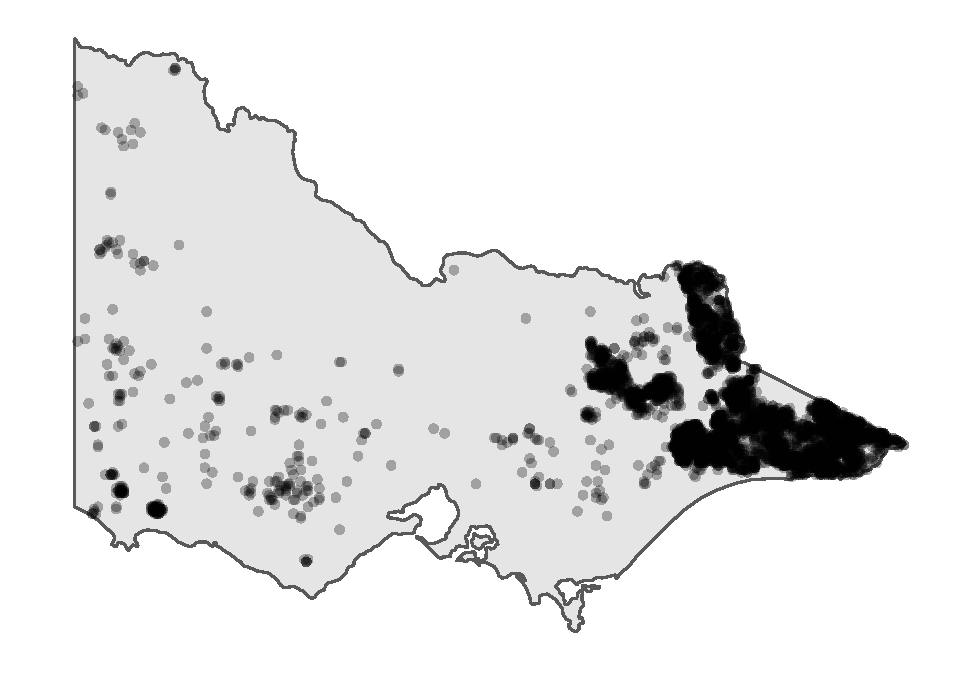
\includegraphics[width=0.8\linewidth]{clustering_paper_files/figure-latex/hotspots-1} \caption[Hotspot locations in Victoria during 2019-2020 season]{Hotspot locations in Victoria during 2019-2020 season.}\label{fig:hotspots}
\end{figure}
\end{Schunk}

\hypertarget{steps}{%
\subsubsection{Steps}\label{steps}}

This algorithm runs in a temporal manner. Starting from the first hour
of the first day or the bushfire season, hotspots are grouped, and then
agglomerated spatially. This proceeds to the next hour.

\textbf{1. Divide hotspots by hour}

Show faceted plots of hotspot data (from full map) for first five hours,
all in one row of plots

Hour is used as the basic unit of time, to simplify the computation, but
it could be a different time resolution.

\textbf{2. Start from the first hour}

Plot of one hour, small area, so we can show how the algorithm does
grouping

It first selected entries of the first timestamps, which was the first
hour in the hotspots data.

\textbf{3. Connect adjacent hotspots and active centroids (3km)}

Show connection of points from previous plot

The algorithm then calculated the matrix of pairwise geodesic distances
between all points being selected. With the geodesic distances matrix,
an ``adjacent distance'' as one of the hyperparameters in this algorithm
was used to determine the adjacency matrix. If a geodesic distance
between two points was less than the ``adjacent distance'', the
corresponding entry in the adjacency matrix would be assigned with
integer 1, otherwise it would be assigned with integer 0. Normally, this
``adjacent distance'' would be set between 0 to 100000 meters. Using the
adjacency matrix, the algorithm then constructed a undirected unweighted
graph. For each connected component in this graph, a unique integer was
assigned as the membership. In our hotspots data, components could be
recognised as bushfires. Points in the same component shared with the
same membership.

\textbf{4. For each point, if there is a connected nearest active
centroid, join its group}

Meanwhile, the longitude and the latitude of centroids in each component
were calculated by taking the average of longitude and the average of
latitude for all points in the corresponding component. Those centroids
along with memberships would then be recorded and labelled as active
groups. In other words, their ``active'' attributes were assigned with
integer 0.

\textbf{5. Otherwise, create a new group for each connected graph}

Show grouped observations

\textbf{6. Compute centroid for each group}

Show centroids

\textbf{7. Keep the group active until there is no new hotspots join the
group within 24 hours}

When the algorithm moved to the next timestamps, it subtracted 1 from
``active'' attributes. Another hyperparameter ``group active time'' was
used for selecting active groups. Conventionally, ``group active time''
was set to be 24 hours. If any centroid had an ``active'' attribute
greater than the negative of ``group active time'', it would be selected
as active groups.

For the second and the later timestamps, the algorithm first combined
centroids of active groups with the hotspots data in the corresponding
timestamps. It then calculated geodesic distances matrix, filled
adjacency matrix and constructed graph as before. There was an
additional step which was to find the nearest active group within the
same component for each point. If a point shared the same component with
active groups, it would be assigned with the membership of the nearest
active group. Otherwise, points shared with the same component would be
assigned with a new membership. Therefore, points in one component would
not necessary had the same membership if there were more than one active
groups within a component. All centroids of active groups and new group
would then be recalculated and updated using only the current timestamps
hotspots data. Their ``active'' attributes were set to be 0.

This algorithm worked till the last timestamps. The end result was a
vector of memberships with length equal to number of rows in hotspots
data and a time-series record of all groups.

For computational performance, we stored the hostpots data in a SQLite
database. Relevant operation was done by using packages \texttt{DBI} and
\texttt{RSQLite}. Geodesic distances matrix was calculated using package
\texttt{geodist}. Graph operation was done by using package
\texttt{igraph}.

\textbf{8. Repeat this process to the last hour}

The code implemented this algorithm is ``clustering.R''.

\hypertarget{effects-of-parameter-choices}{%
\subsubsection{Effects of parameter
choices}\label{effects-of-parameter-choices}}

There are two parameters that can be tuned in this algorithm. They are
\texttt{adj\_dist}, which is the density distance and
\texttt{active\_time}, which is the .

\begin{Schunk}
\begin{figure}
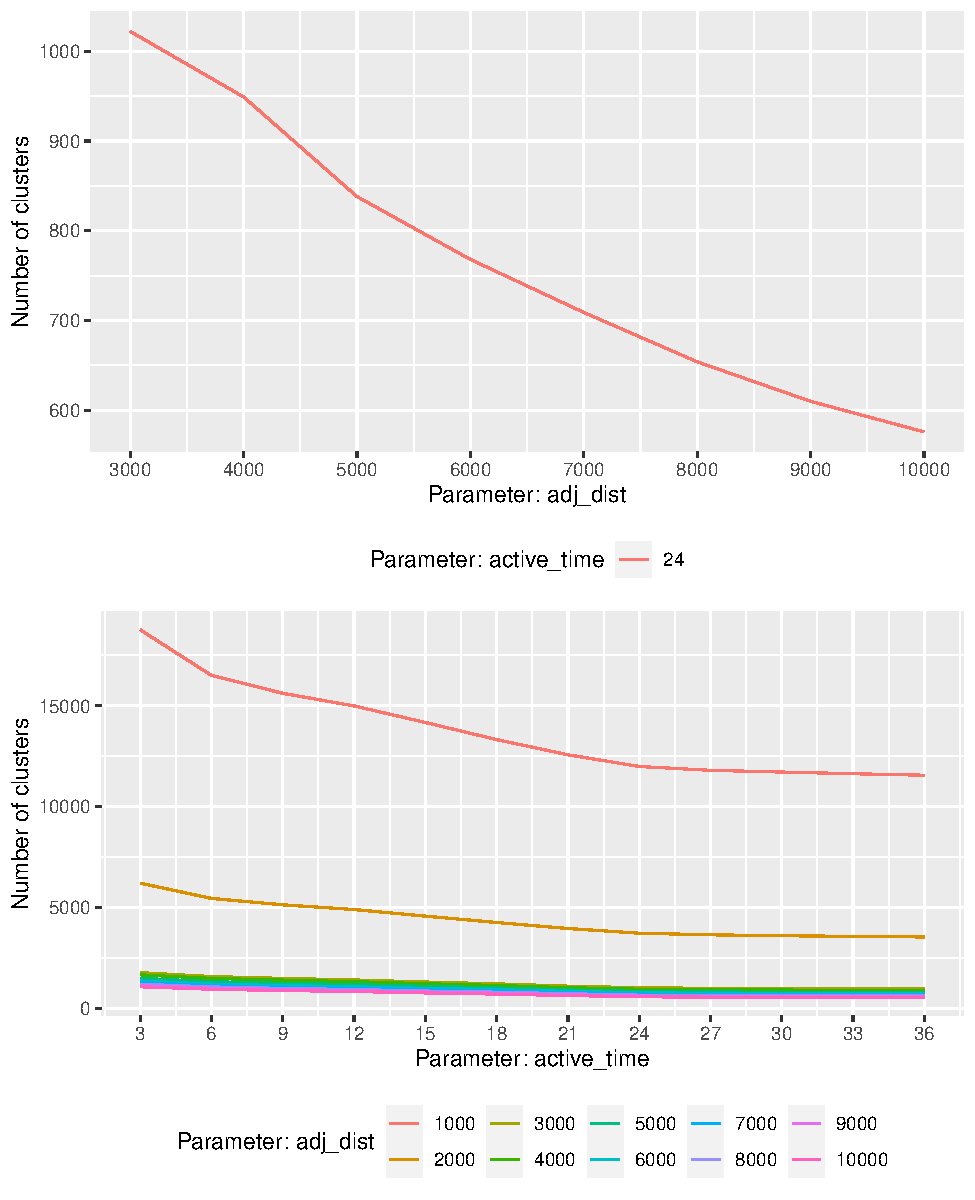
\includegraphics[width=0.8\linewidth]{clustering_paper_files/figure-latex/para_1-1} \caption[Number of clusters under different parameter choices]{Number of clusters under different parameter choices}\label{fig:para_1}
\end{figure}
\end{Schunk}

\hypertarget{application}{%
\subsection{Application}\label{application}}

\hypertarget{determining-the-ignition-point-and-time-for-individual-fires}{%
\subsubsection{Determining the ignition point and time for individual
fires}\label{determining-the-ignition-point-and-time-for-individual-fires}}

Show ignition points for a particularly heavy day and another for a
particularly light day

\begin{Schunk}

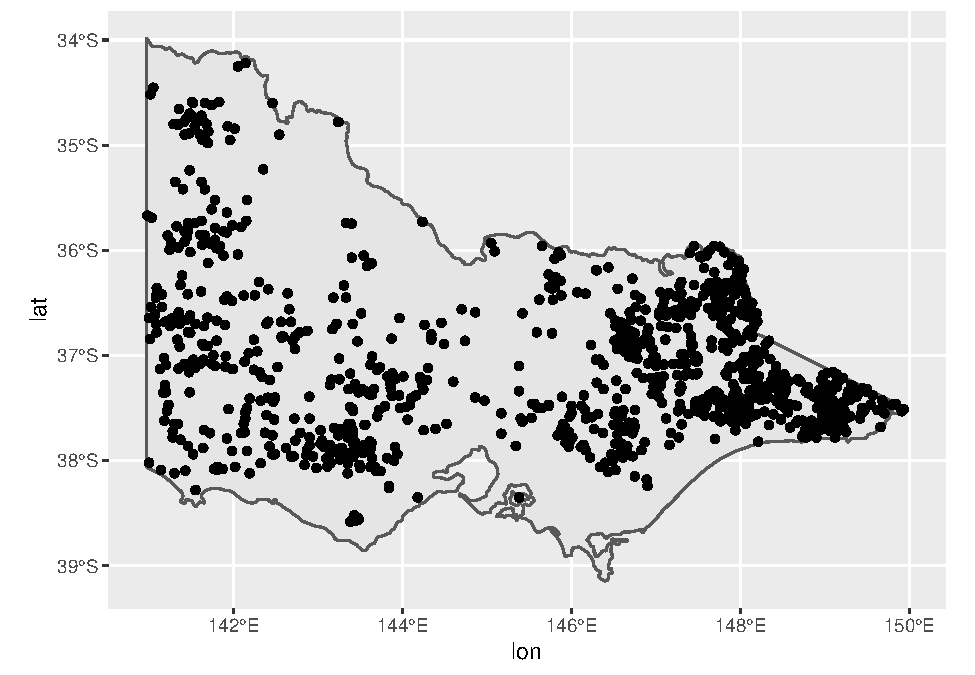
\includegraphics[width=0.8\linewidth]{clustering_paper_files/figure-latex/unnamed-chunk-2-1} \end{Schunk}

\begin{Schunk}

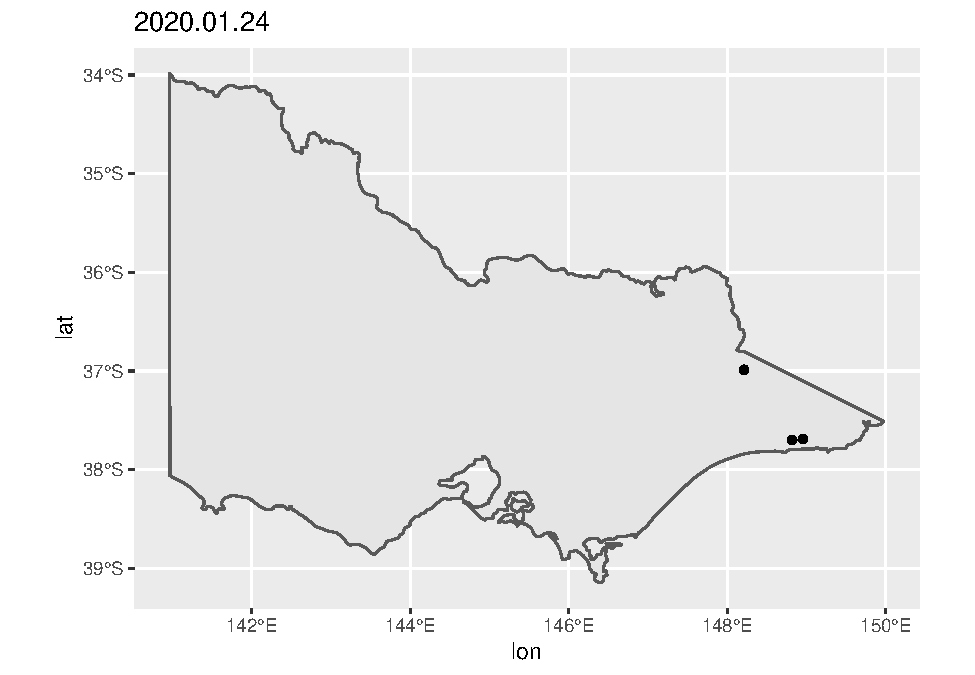
\includegraphics[width=0.8\linewidth]{clustering_paper_files/figure-latex/unnamed-chunk-4-1} \end{Schunk}

\begin{Schunk}

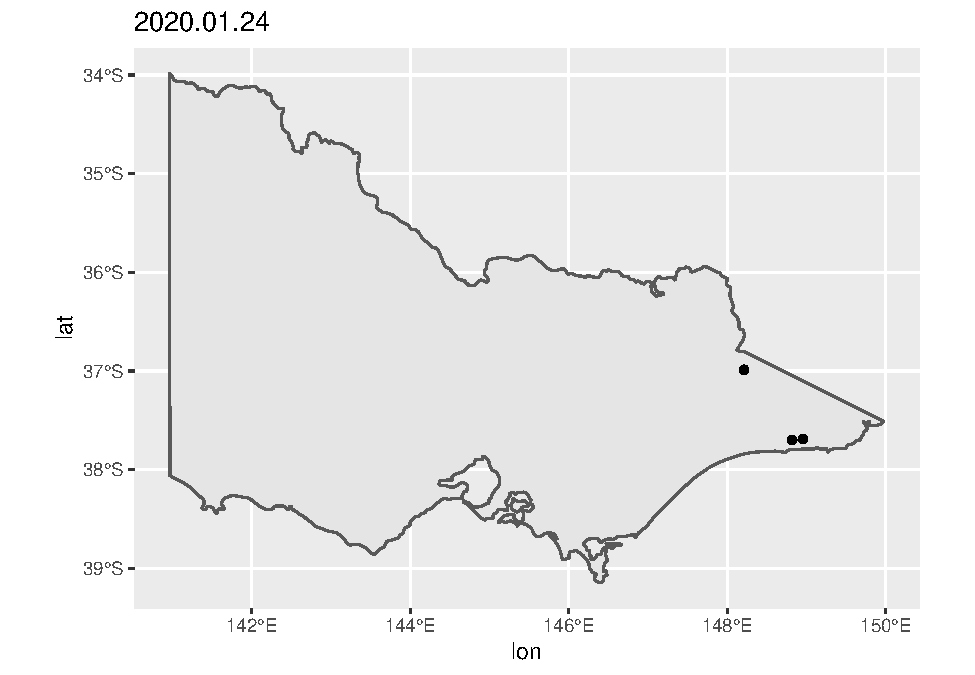
\includegraphics[width=0.8\linewidth]{clustering_paper_files/figure-latex/unnamed-chunk-5-1} \end{Schunk}

\hypertarget{tracking-fire-movement}{%
\subsubsection{Tracking fire movement}\label{tracking-fire-movement}}

Display showing how a fire moves over time, maybe two or more fires

\hypertarget{allocating-resources-for-future-fire-prevention}{%
\subsubsection{Allocating resources for future fire
prevention}\label{allocating-resources-for-future-fire-prevention}}

Merging data with camp sites, CFA, roads, \ldots{}

\hypertarget{summary}{%
\subsection{Summary}\label{summary}}

\hypertarget{acknowledgements}{%
\subsection{Acknowledgements}\label{acknowledgements}}

\begin{itemize}
\tightlist
\item
  The code and files to reproduce this work are at XXX
\item
  Data on hotspots can be downloaded from XXX
\end{itemize}

\bibliography{RJreferences}


\address{%
Weihao Li\\
Monash University\\%
line 1\\ line 2\\
%
%
%
\\\href{mailto:wlii0039@student.monash.edu}{\nolinkurl{wlii0039@student.monash.edu}}
}

\address{%
Emily Dodwell\\
AT\&T\\%
line 1\\ line 2\\
%
%
%
\\\href{mailto:emily@research.att.com}{\nolinkurl{emily@research.att.com}}
}

\address{%
Dianne Cook\\
Monash University\\%
line 1\\ line 2\\
%
%
%
\\\href{mailto:dicook@monash.edu}{\nolinkurl{dicook@monash.edu}}
}

